\documentclass[12pt,a4paper]{report}

% ============================ 预加载的 LaTeX 包 ============================
\usepackage[a4paper,left=3.5cm,right=3cm,top=3cm,bottom=3cm]{geometry} % 页面边距
\usepackage[protrusion=true,expansion=true]{microtype}  % 细节优化
\usepackage{setspace}                         % 设置 1.5 倍行距
\usepackage{fancyhdr}                         % 自定义页眉页脚
\usepackage{newtxtext,newtxmath}              % 设置 Times New Roman 字体
\usepackage{amsmath, amssymb, amsthm}         % 数学支持
\usepackage{graphicx}                         % 插入图片
\usepackage{hyperref}                         % 目录超链接
\usepackage{booktabs}                         % 美化表格
\usepackage{array}                            % 处理表格对齐
\usepackage{multicol}                         % 多列布局
\usepackage[toc,page]{appendix}               % 处理附录
\usepackage{tocbibind}  % 让目录中包含“参考文献”和“附录”
\usepackage{caption}                          % 处理表格和图片标题格式
\usepackage{xcolor}                           % 颜色支持
\usepackage{titlesec}                         % 控制标题字体大小
\usepackage{eso-pic}                          % 添加水印
\usepackage{tikz}                             % 让水印精确定位
\usepackage{datetime}                         % 格式化日期
\usepackage{tocloft}                          % 目录格式控制
\usepackage{titlesec}                         % 标题格式控制
\usepackage{titletoc}                         % 目录格式增强
\usepackage{cite}                             % bib引用
\usepackage{lipsum}                           % 内容模拟
% \usepackage{showframe}

% ================================= 设置页脚 ================================
\pagestyle{fancy}                                         % 启用 fancyhdr
\fancyhf{}                                                % 清除默认的页眉和页脚
\fancyfoot[R]{\fontsize{12pt}{14pt}\selectfont \thepage}  % 右侧页脚页码 12pt
\renewcommand{\headrulewidth}{0pt}                        % 取消页眉下划线
\renewcommand{\footrulewidth}{0pt}                        % 取消页脚下划线
\fancypagestyle{plain}{                                   % 适配plain风格页面
    \fancyhf{} 
    \fancyfoot[R]{\fontsize{12pt}{14pt}\selectfont \thepage}
    \renewcommand{\headrulewidth}{0pt}
    \renewcommand{\footrulewidth}{0pt}
}

% ================================= 设置目录 ================================
% 修改目录标题格式(居中 + 18pt + 加粗 + 下划线)
\renewcommand{\contentsname}{}
\newcommand{\customtoc}{
    \clearpage
    \begin{center}
        \underline{\textbf{\fontsize{18pt}{18pt}\selectfont Table of Contents}}
    \end{center}
    \vspace{-1.2\baselineskip}
}
% 自定义 "Pages" 列标题,使其右对齐
\renewcommand{\cftaftertoctitle}{%
    \vspace{-1.5\baselineskip} % 减少 Table of Contents 后的额外空行
    \hfill\underline{Pages} % 右对齐
    \par\vskip-2\baselineskip % 调整间距,防止错位
}
%目录格式调整
% 一级标题 (chapter) 设置
\renewcommand{\cftchapfont}{\bfseries}                  % 章节标题加粗
\renewcommand\thechapter{Chapter\enspace\arabic{chapter}}       % 添加 "Chapter " 前缀
\renewcommand\thesection{\arabic{chapter}.\arabic{section}} % 解决上行代码的乱码问题
\renewcommand{\cftchapaftersnumb}{}                     % 章节编号后不添加任何内容
\setlength{\cftchapnumwidth}{5.3em}                       % 设置编号宽度
% 二级标题(section)设置
\renewcommand{\cftsecfont}{}                            % 节标题字体
\renewcommand{\cftsecpresnum}{}                         % 节编号前缀
\renewcommand{\cftsecaftersnumb}{}                      % 节编号后缀
\setlength{\cftsecindent}{0em}                          % 节的缩进
\setlength{\cftsecnumwidth}{2em}                        % 节编号宽度
\renewcommand{\cftsecdotsep}{\cftnodots}                % 移除点线
\renewcommand{\cftsecpagefont}[1]{}                     % 移除页码
% 间距设置
\setlength{\cftbeforechapskip}{0.5em}                   % 章节前的间距
\setlength{\cftbeforesecskip}{0.5em}                    % 节前的间距

% ========================== 统一设置 \chapter ==========================
% 设置有编号的 \chapter 显示 "Chapter 1" + 换行后的标题左对齐
\titleformat{\chapter}[display]            % "Chapter 1" 独立一行,标题换行后左对齐
  {\normalfont\Huge\bfseries}  % 不倾斜,字号 Huge,加粗
  {\thechapter}                            % 显示 "Chapter 1"
  {0em}                                    % 章节编号和标题之间的间距
  {\raggedright}                           % 标题居左
% 设置无编号的 \chapter*{}(如摘要、附录等)格式,不带 "Chapter"
\titleformat{name=\chapter,numberless}[display]
  {\normalfont\Huge\bfseries}  % 不倾斜,字号 Huge,加粗
  {}                                       % 无编号时不显示 "Chapter 1"
  {-2.5em}                                 % 章节编号和标题之间的间距
  {\centering}                             % 标题居中
% 调整章节标题的间距
\titlespacing{\chapter}{0pt}{-2em}{0em}  % 影响有编号的章节
\titlespacing{name=\chapter,numberless}{0pt}{0em}{\baselineskip}  % 影响无编号的章节

% ========================== 统一设置 \section ==========================
% 设置有编号的 \section{}
\titleformat{\section}                        % 统一设置 section
  {\normalfont\fontsize{16pt}{16pt}\bfseries} % 12pt 字号行距,加粗
  {\thesection\enspace}                       % 章节编号(这里为空)
  {0pt}                                       % 章节前间距
  {\raggedright}                              % 章节后格式(这里保持默认)
% 设置无编号的 \section*{}
\titleformat{name=\section,numberless}[display]
  {\clearpage\normalfont\fontsize{16pt}{16pt}\bfseries}
  {}
  {-1em}
  {\centering}
\titlespacing{\section}{0pt}{0.5\baselineskip}{0.5\baselineskip}
\titlespacing{name=\section,numberless}{0pt}{0em}{1.5\baselineskip}

\global\sloppy  % 允许换行,减少溢出

\begin{document}

\onehalfspacing % 1.5 倍行距

% ================================ 自定义颜色 ================================
\definecolor{DeepGreen}{rgb}{0.0, 0.690, 0.314}

% ================================ 自定义设置 ================================
% 左缩进为0
\setlength{\parindent}{0pt}
% 自定义日期格式
\newdateformat{mydate}{\THEDAY\ \monthname[\THEMONTH]\ \THEYEAR}
% 让图编号显示为 "Figure X.Y"
\renewcommand{\thefigure}{Figure \arabic{chapter}.\arabic{figure}}
\setlength{\cftfignumwidth}{4.5em}
\renewcommand{\figurename}{}
% 调整 listoffigures (图目录) 的格式
\makeatletter
\renewcommand{\listoffigures}{%
    \begingroup
    \vspace{-2em} % 减少上方间距
    \chapter*{\listfigurename}%
    \@starttoc{lof}%
    \endgroup
}
\makeatother
% 让表格编号显示为 "Table X.Y"
\renewcommand{\thetable}{Table \arabic{chapter}.\arabic{table}}
\setlength{\cfttabnumwidth}{4.5em}
\renewcommand{\tablename}{}
% 调整 listoftables (表目录) 的格式
\makeatletter
\renewcommand{\listoftables}{%
    \begingroup
    \vspace{-2em} % 减少上方间距
    \chapter*{\listtablename}%
    \@starttoc{lot}%
    \endgroup
}
\makeatother


% ======================== 论文前置部分(Front Matter) =======================
\pagenumbering{gobble}
\begin{titlepage}
    \centering
    
    % 第一页
    \vspace*{1cm}
    
    
\includegraphics[width=0.8\textwidth]{assets/ntu-logo.png} % NTU Logo
    
    \vspace*{6cm}
    
    \textbf{\LARGE{\textcolor{red}{DISSERTATION TITLE}}}
    
    \vfill
    
    \textbf{\textcolor{red}{AUTHOR'S NAME}} \\
    \textbf{SCHOOL OF ELECTRICAL AND ELECTRONIC ENGINEERING} \\
    \textbf{\textcolor{red}{2025}}

    \vspace*{1cm}

    % 第二页
    \newpage
    
    \vspace*{6cm}
    
    \textbf{\LARGE{\textcolor{red}{DISSERTATION TITLE}}}

    \vspace*{6cm}

    \textbf{\textcolor{red}{AUTHOR’S NAME}}

    \vspace*{2cm}

    \textbf{SCHOOL OF ELECTRICAL AND ELECTRONIC ENGINEERING}

    \vspace*{\baselineskip}

    \textbf{A DISSERTATION SUBMITTED IN PARTIAL FULFILMENT OF THE REQUIREMENTS FOR THE DEGREE OF} \\
    \textbf{MASTER OF SCIENCE IN} \\
    \textbf{\textcolor{red}{SIGNAL PROCESSING AND MACHINE LEARNING}}

    \vfill

    \textbf{\textcolor{red}{2025}}

    \vspace*{1cm}
\end{titlepage}             % 论文封面
\section*{Statement of Originality}

I hereby certify that the work embodied in this thesis is the result of original research, is free of plagiarised materials, and has not been submitted for a higher degree to any other University or Institution.

\vspace*{1cm}

\noindent
\begin{center} % 让整个表格居中
    \begin{tabular}{>{\centering\arraybackslash}p{6cm} p{1cm} >{\centering\arraybackslash}p{6cm}} % 居中对齐
        \mydate\today &  & 
        \begin{tikzpicture} % 签名&水印
            \node[opacity=0.9, anchor=center] at (0,0) {
\includegraphics[width=5cm]{assets/ntu-watermark.png}};
            % 在水印上方插入手写签名图片
            \node[anchor=north] at (0,2) {
\includegraphics[width=4cm]{signature/personal-signature.png}};
        \end{tikzpicture} \\ % 第一行:日期和签名水印
        \dotfill &  & \dotfill \\[0.2cm] % 第二行:虚线
        Date &  & \textcolor{red}{Your Name} \\ % 第三行:日期说明 & 姓名
    \end{tabular}
\end{center}
            % 原创性声明
\section*{Supervisor Declaration Statement}
I have reviewed the content and presentation style of this thesis and declare it is free of plagiarism and of sufficient grammatical clarity to be examined. To the best of my knowledge, the research and writing are those of the candidate except as acknowledged in the Author Attribution Statement. I confirm that the investigations were conducted in accord with the ethics policies and integrity standards of Nanyang Technological University and that the research data are presented honestly and without prejudice.

\vspace*{1cm}

\noindent
\begin{center} % 让整个表格居中
    \begin{tabular}{>{\centering\arraybackslash}p{6cm} p{1cm} >{\centering\arraybackslash}p{6cm}} % 居中对齐
        \mydate\today &  & 
        \begin{tikzpicture} % 签名&水印
            \node[opacity=0.9, anchor=center] at (0,0) {
\includegraphics[width=5cm]{assets/ntu-watermark.png}};
            % 在水印上方插入手写签名图片
            \node[anchor=north] at (0,2) {
\includegraphics[width=4cm]{signature/personal-signature.png}};
        \end{tikzpicture} \\ % 第一行:日期和签名水印
        \dotfill &  & \dotfill \\[0.2cm] % 第二行:虚线
        Date &  & \textcolor{red}{Supervisor Name} \\ % 第三行:日期说明 & 姓名
    \end{tabular}
\end{center} % 导师声明
\section*{Authorship Attribution Statement}

Please select one of the following; *delete as appropriate:

\vspace{0.5\baselineskip}

*(A) This thesis does not contain any materials from papers published in peer-reviewed journals or from papers accepted at conferences in which I am listed as an author.

\vspace{0.5\baselineskip}

*(B) This thesis contains material from [x number] paper(s) published in the following peer-reviewed journal(s) / from papers accepted at conferences in which I am listed as an author.

\vspace{0.5\baselineskip}

\textcolor{DeepGreen}{\underline{
Please amend the typical statements below to suit your circumstances if (B) is selected.
}}

\vspace{0.5\baselineskip}

Chapter 4 is published as: 
\textcolor{DeepGreen}{
D.T. Murphy, S. Schmid, J.R. Hester, P.E.R. Blanchard, and W. Miiller. Coordination site disorder in spinel-type LiMnTiO₄. \textit{Inorganic Chemistry} 54, 4636-4643 (2015). DOI: \href{https://doi.org/10.1021/ic502747p}{10.1021/ic502747p}.
}

\vspace{0.5\baselineskip}

The contributions of the co-authors are as follows:

\begin{itemize}
    \setlength\parskip{0pt} % 彻底去除 itemize 前后的额外间距
    \item \textcolor{DeepGreen}{A/Prof Schmid provided the initial project direction and edited the manuscript drafts.}
    \item \textcolor{DeepGreen}{I prepared the manuscript drafts. The manuscript was revised by Dr Hester and Dr. Blanchard.}
    \item \textcolor{DeepGreen}{I co-designed the study with A/Prof Siegbert Schmid and performed all the laboratory work at the School of Materials Science and Engineering and the Singapore Synchrotron Light Source. I also analyzed the data.}
    \item \textcolor{DeepGreen}{All microscopy, including sample preparation, was conducted by me in the Facility for Analysis, Characterization, Testing and Simulation.}
    \item \textcolor{DeepGreen}{Dr James Hester assisted in the collection of the neutron powder diffraction data.}
    \item \textcolor{DeepGreen}{Dr Peter Blanchard assisted in the interpretation of the X-ray absorption spectroscopy data and carried out the spectral interpretation.}
    \item \textcolor{DeepGreen}{Dr Wojciech Miiller assisted in the collection and provided guidance in the interpretation of the magnetic measurement data.}
\end{itemize}


Chapter 5 is published as:
\textcolor{DeepGreen}{
H. V Doan, B. Yao, Y. Fang, A. Sartbaeva, U. Hintermair, V. P Ting, Controlled Formation of Hierarchical Metal-Organic Frameworks using CO₂ Expanded Solvent Systems. \textit{ACS Sustainable Chemistry \& Engineering} (2017). DOI: \href{https://doi.org/10.1021/acssuschemeng.7b01429}{10.1021/acssuschemeng.7b01429}.
}

\vspace{1cm}

The contributions of the co-authors are as follows:

\begin{itemize}
    \setlength\parskip{0pt} % 彻底去除 itemize 前后的额外间距
    \item \textcolor{DeepGreen}{Prof Ting suggested the materials area and edited the manuscript drafts.}
    \item 
    \textcolor{DeepGreen}{I performed all the materials synthesis, collected X-ray diffraction patterns and visible light spectra, carried transmission electron microscopy, and conducted data evaluation.}
    \item 
    \textcolor{DeepGreen}{I performed all the materials synthesis, collected X-ray diffraction patterns and visible light spectra, carried transmission electron microscopy, and conducted data evaluation.}
    \item 
    \textcolor{DeepGreen}{Dr. Y. Fang conducted the Rietveld analysis of the powder X-ray diffraction data and single crystal structure determinations.}
    \item 
    \textcolor{DeepGreen}{Dr U. Hintermair conducted the molecular dynamics simulations.}
    \item 
    \textcolor{DeepGreen}{Ms. A. Sartbaeva prepared the samples for electron microscopy.}
\end{itemize}

\vspace*{1cm}

\noindent
\begin{center} % 让整个表格居中
    \begin{tabular}{>{\centering\arraybackslash}p{6cm} p{1cm} >{\centering\arraybackslash}p{6cm}} % 居中对齐
        \mydate\today &  & 
        \begin{tikzpicture} % 签名&水印
            \node[opacity=0.9, anchor=center] at (0,0) {
\includegraphics[width=5cm]{assets/ntu-watermark.png}};
            % 在水印上方插入手写签名图片
            \node[anchor=north] at (0,2) {
\includegraphics[width=4cm]{signature/personal-signature.png}};
        \end{tikzpicture} \\ % 第一行:日期和签名水印
        \dotfill &  & \dotfill \\[0.2cm] % 第二行:虚线
        Date &  & \textcolor{red}{Your Name} \\ % 第三行:日期说明 & 姓名
    \end{tabular}
\end{center}
             % 著作声明

\clearpage
\centering\customtoc
\addtocontents{toc}{\protect\setcounter{tocdepth}{-1}} % 暂时隐藏目录
\tableofcontents % 生成目录
\addtocontents{toc}{\protect\setcounter{tocdepth}{2}}  % 恢复目录
\clearpage

\clearpage
\pagenumbering{roman}                         % 正文前使用罗马数字编号
\setcounter{page}{1}                          % 从 i 开始
\pagestyle{fancy}                             % 确保页码继续显示在右侧页脚
\chapter*{Abstract}
\addcontentsline{toc}{chapter}{Abstract}
\begingroup
\justifying
\setlength{\parindent}{0pt}
\setstretch{2} % 设置为2的时候为word1.5倍行距
\setlength{\parskip}{0.5\baselineskip}

Multihop cellular networks (MCNs) incorporate wireless ad hoc networking into traditional single-hop cellular networks (SCNs) and thus they enjoy the flexibility of ad hoc networks, while preserving the benefit of using infrastructure of SCNs. In this Thesis, we study the resource allocation problems in MCNs.

Multihop cellular networks (MCNs) incorporate wireless ad hoc networking into traditional single-hop cellular networks (SCNs) and thus they enjoy the flexibility of ad hoc networks, while preserving the benefit of using infrastructure of SCNs. In this Thesis, we study the resource allocation problems in MCNs.

\endgroup               % 摘要
\chapter*{Acknowledgement (optional)}
\addcontentsline{toc}{chapter}{Acknowledgement (optional)}
\begingroup
\raggedright
\setstretch{2} % 设置为2的时候为word1.5倍行距
\setlength{\parskip}{0.5\baselineskip}

First of all, I would like to express my sincere thanks and great gratitude to my parents. ...

\begin{flushright}
Your name \\
\mydate\today
\end{flushright}

\endgroup        % 致谢(可选)
% \chapter*{Acronyms (optional)}
% \addcontentsline{toc}{chapter}{Acronyms (optional)}

% \noindent
% \begin{tabular}{ll} % 两列表格
% 2G & Second Generation \\
% 3G & Third Generation \\
% ACA & Adaptive Channel Assignment \\
% AP & Access Point \\
% ARS & Ad-hoc Relaying Station \\
% ASP & Adaptive Switching Point \\
% ATDMA & Advanced Time Division Multiple Access \\
% BS & Base Station \\
% CAMA & Cellular Aided Mobile Ad-hoc Network \\
% CBM & Cellular Based Multihop Systems \\
% CDD & Code-Division Duplexing \\
% D-PRMA & Distributed PRMA \\
% DA & Demand Assignment \\
% DCA & Dynamic Channel Assignment \\
% \end{tabular}

\chapter*{Acronyms}

\addcontentsline{toc}{chapter}{Acronyms}

\noindent
\begin{tabular}{ll} % 两列表格
CNN & Convolutional Neural Network \\
DLO & Deformable Linear Objects \\
DOM & Deformable Object Manipulation \\
YOLO & You Only Look Once \\
YOLO11 & You Only Look Once version 11 \\
BBOX & Bounding Box \\
OBB  & Oriented Bounding Box \\
\end{tabular}               % 术语缩写表(可选)
\chapter*{Symbols (optional)}
\addcontentsline{toc}{chapter}{Symbols (optional)}

\noindent
\begin{tabular}{ll} % 两列对齐
B & channel bandwidth in Hz \\
C & channel capacity in bps; \\
  & number of collisions in time slot $t$ \\
d & distance \\
D & minimum reuse distance \\
$D_a$ & average message access delay \\
$D_{id}$ & inter-datagram-arrival time \\
$D_{max}$ & maximum tolerable delay for voice packets \\
\end{tabular}                % 符号表(可选)
\listoffigures                                % 生成图目录
\listoftables                                 % 生成表目录

% ========================= 论文正文部分(Main Content) ========================
\clearpage
\pagenumbering{arabic}       % 正文部分改为阿拉伯数字
\setcounter{page}{1}         % 从 1 开始
\pagestyle{fancy}            % 确保页码继续显示在右侧页脚
\chapter{Introduction}
\begingroup
\raggedright
\setstretch{2}
\setlength{\parskip}{0.5\baselineskip}
\titlespacing{\chapter}{0pt}{0pt}{0pt}
\titlespacing{\section}{0pt}{0pt}{0pt}

This chapter \lipsum[1]

\section{Motivations}

This thesis deals with the problem of the blind multiuser detection for DS-CDMA. This thesis deals with the problem of the blind multiuser detection for DS-CDMA...

\lipsum[1-2]

\section{Objectives and Scope}

The communication channel considered in this thesis is assumed to be slow time-varying. \lipsum[1]

Wireless communication is evolving rapidly \cite{jordan2002,padgett1995}.

\section{Organisation}

\lipsum[1-2]

\begin{figure}[h]
    \centering
    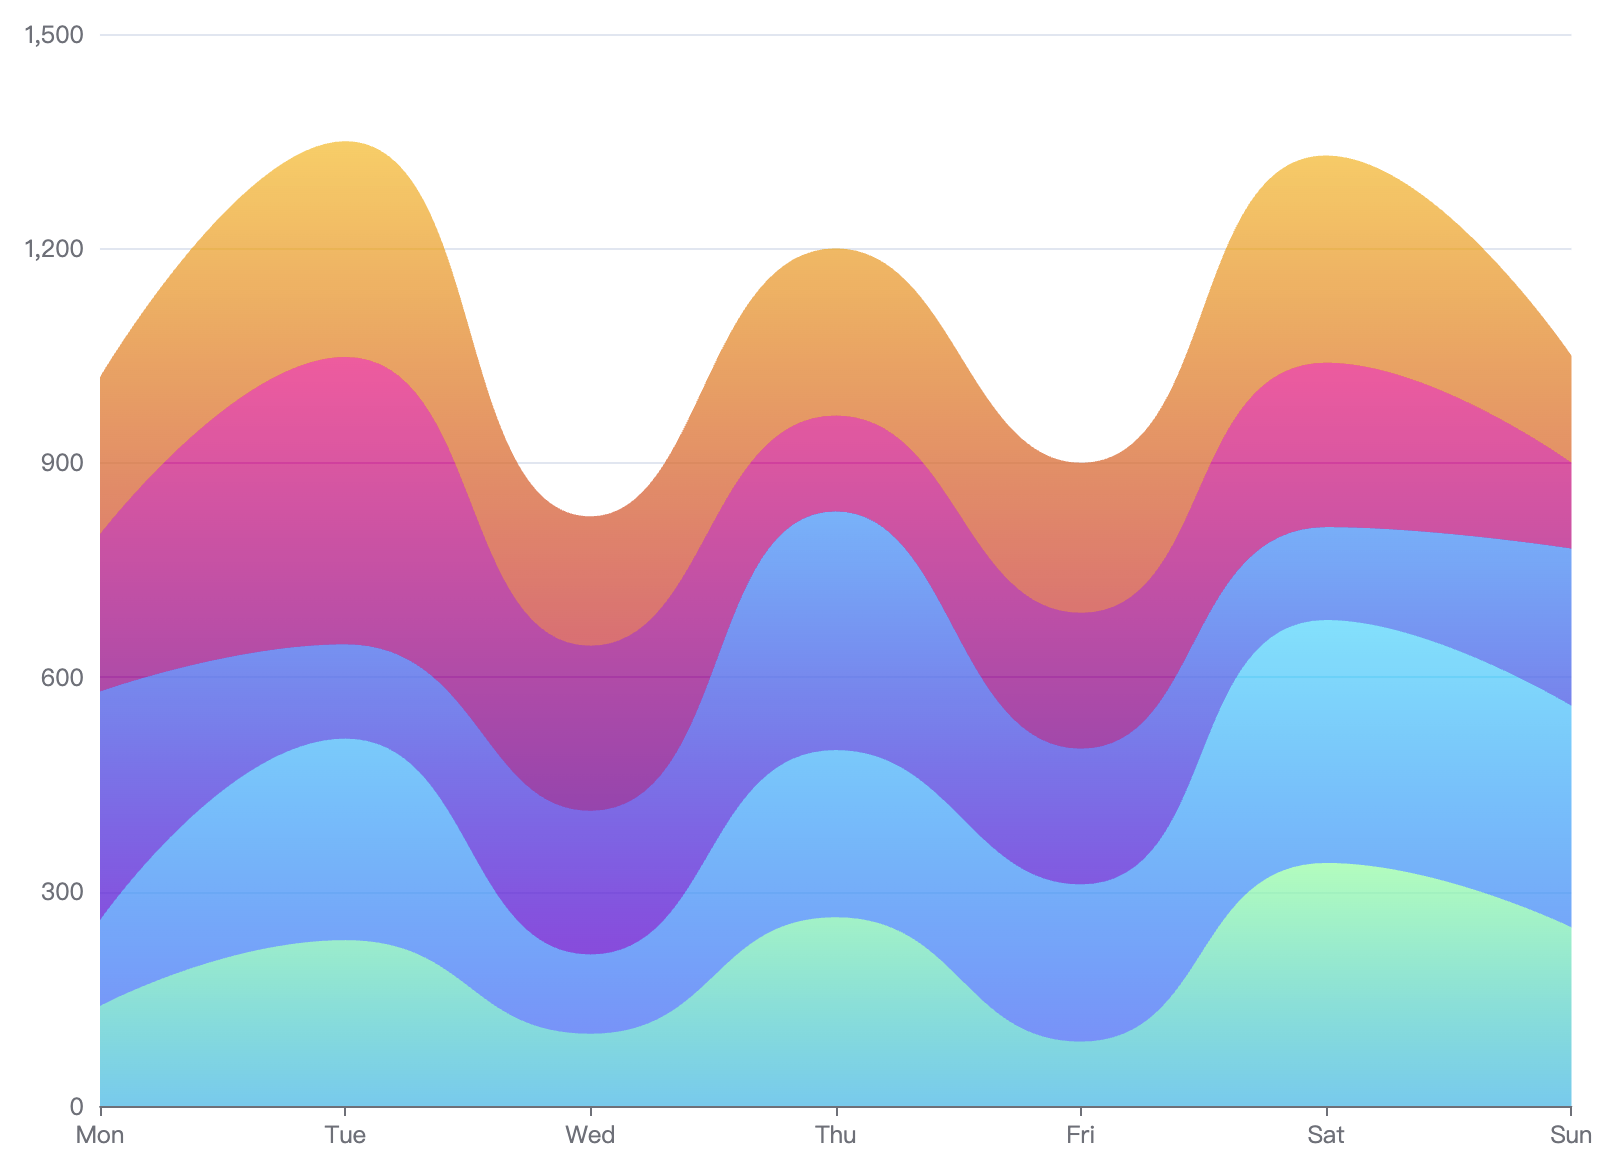
\includegraphics[width=0.6\textwidth]{assets/figures/demo.png}
    \caption{Proposed CMCN architecture}
    \label{fig:cmcn}
\end{figure}

\endgroup  % 第一章
\chapter{Literature Review}
\begingroup
\justifying
\setlength{\parindent}{0pt}
\setstretch{2}
\setlength{\parskip}{0.5\baselineskip}
\titlespacing{\chapter}{0pt}{0pt}{0pt}
\titlespacing{\section}{0pt}{0pt}{0pt}

\section{xxx}
\section{xxx}
\section{xxx}

\endgroup  % 第二章
\chapter{XXX}
\begingroup
\raggedright
\setstretch{2}
\setlength{\parskip}{0.5\baselineskip}
\titlespacing{\chapter}{0pt}{0pt}{0pt}
\titlespacing{\section}{0pt}{0pt}{0pt}

\section{xxx}
\section{xxx}
\section{xxx}

\endgroup  % 第三章
\chapter{XXX}
\begingroup
\raggedright
\setstretch{2}
\setlength{\parskip}{0.5\baselineskip}
\titlespacing{\chapter}{0pt}{0pt}{0pt}
\titlespacing{\section}{0pt}{0pt}{0pt}

\section{xxx}
\section{xxx}
\section{xxx}

\endgroup  % 第四章
\chapter{XXX}
\begingroup
\raggedright
\setstretch{2}
\setlength{\parskip}{0.5\baselineskip}
\titlespacing{\chapter}{0pt}{0pt}{0pt}
\titlespacing{\section}{0pt}{0pt}{0pt}

\section{xxx}
\section{xxx}
\section{xxx}

\endgroup  % 第五章
\chapter{Conclusions and Future Work}

\begingroup
\justifying
\setlength{\parindent}{0pt}
\setstretch{2}
\setlength{\parskip}{0.5\baselineskip}
\titlespacing{\chapter}{0pt}{0pt}{0pt}
\titlespacing{\section}{0pt}{0pt}{0pt}

\section{Conclusions}

\begin{table}[h]
    \centering
    \caption{Example Table Title}
    \label{tab:example}
    \begin{tabular}{|c|c|c|}
        \hline
        Column 1 & Column 2 & Column 3 \\ \hline
        Data 1   & Data 2   & Data 3   \\ \hline
        Data 4   & Data 5   & Data 6   \\ \hline
        Data 7   & Data 8   & Data 9   \\ \hline
    \end{tabular}
\end{table}

\section{Recommendation in Future Work}

\endgroup  % 第六章

% ============================ 参考文献(References) ===========================
% thebibliography管理References
% 选此方式保留references.tex,删除references.bib
\begingroup
\renewcommand{\chapter}[2]{}  % 禁止 thebibliography 自动添加目录项
\endgroup
\renewcommand{\bibname}{References}
\chapter*{\makebox[\textwidth][l]{\bibname}}

\begingroup
\renewcommand{\chapter}[2]{}  % 禁止 thebibliography 自动添加目录项
\begin{thebibliography}{9}
    \bibitem{jordan2002} R. Jordan and C. T. Abdallah, "Wireless communications and networking: An overview," IEEE Antennas and Propagation Magazine, vol. 44, pp. 185-193, February, 2002.
    \bibitem{padgett1995} J. E. Padgett, C. G. Gunther, and T. H. Hattori, "Overview of wireless personal communications," IEEE Communications Magazine, vol. 33, pp. 28-41, January, 1995.
\end{thebibliography}
\endgroup
% bib格式管理References
% 选此方式保留references.bib,删除references.tex
% \renewcommand\bibsection{\chapter*{\makebox[\textwidth][l]{\bibname}}}
% \bibliographystyle{IEEEtran}             % 指定 IEEE 风格
% \bibliography{c-back-matter/references}  % 你的 .bib 文件(不带 .bib 扩展名)

% ============================== 附录(Appendix) ==============================
\appendix
\chapter*{\makebox[\textwidth][l]{Appendix A (optional)}}
\addcontentsline{toc}{chapter}{Appendix A (optional}
\begingroup
\justifying
\setlength{\parindent}{0pt}
\setstretch{2}
\setlength{\parskip}{0.5\baselineskip}
\titlespacing{\chapter}{0pt}{0pt}{0pt}
\titlespacing{\section}{0pt}{0pt}{0pt}

\lipsum[1-2]

\endgroup % 附录 A
\chapter*{\makebox[\textwidth][l]{Appendix B (optional)}}
\addcontentsline{toc}{chapter}{Appendix B (optional}
\begingroup
\raggedright
\setstretch{2}
\setlength{\parskip}{0.5\baselineskip}
\titlespacing{\chapter}{0pt}{0pt}{0pt}
\titlespacing{\section}{0pt}{0pt}{0pt}

\lipsum[1-2]

\endgroup % 附录 B

\end{document}
